%%%%%%%%%%%%%%%%%%%%%%%%%%%%%%%%%%%%%%%%%%%%%%%%%%%%%%%%%%%%%%%%%%%%%%%%%%%%%%%%
%%%%%%%%%%%%%%%%%%%%%%%%%%%%%%%%%%%%%%%%%%%%%%%%%%%%%%%%%%%%%%%%%%%%%%%%%%%%%%%%
%%% Template for AIMS Rwanda Assignments         %%%              %%%
%%% Author:   AIMS Rwanda tutors                             %%%   ###        %%%
%%% Email: tutors2018-19@aims.ac.rw                               %%%   ###        %%%
%%% Copyright: This template was designed to be used for    %%% #######      %%%
%%% the assignments at AIMS Rwanda during the academic year %%%   ###        %%%
%%% 2018-2019.                                              %%%   #########  %%%
%%% You are free to alter any part of this document for     %%%   ###   ###  %%%
%%% yourself and for distribution.                          %%%   ###   ###  %%%
%%%                                                         %%%              %%%
%%%%%%%%%%%%%%%%%%%%%%%%%%%%%%%%%%%%%%%%%%%%%%%%%%%%%%%%%%%%%%%%%%%%%%%%%%%%%%%%
%%%%%%%%%%%%%%%%%%%%%%%%%%%%%%%%%%%%%%%%%%%%%%%%%%%%%%%%%%%%%%%%%%%%%%%%%%%%%%%%


%%%%%% Ensure that you do not write the questions before each of the solutions because it is not necessary. %%%%%% 

\documentclass[12pt,a4paper]{article}

%%%%%%%%%%%%%%%%%%%%%%%%% packages %%%%%%%%%%%%%%%%%%%%%%%%
\usepackage{amsmath}
\usepackage{amssymb}
\usepackage{amsthm}
\usepackage{amsfonts}
\usepackage{graphicx}
\usepackage[all]{xy}
\usepackage{tikz}
\usepackage{verbatim}
\usepackage[left=2cm,right=2cm,top=3cm,bottom=2.5cm]{geometry}
\usepackage{hyperref}
\usepackage{caption}
\usepackage{subcaption}
\usepackage{psfrag}
\usepackage{multicol}
\usepackage{tabularx}
\usepackage{enumitem}
\usepackage{csvsimple}
\usepackage{booktabs}
\usepackage{colortbl}
\usepackage{tabulary}
\usepackage{etoolbox}

%%%%%%%%%%%%%%%%%%%%% students data %%%%%%%%%%%%%%%%%%%%%%%%
\newcommand{\student}{Kamau Gladys Muthoni}
\newcommand{\course}{Research Methods in Climate Science: FIGURES}
\newcommand{\assignment}{2}

%%%%%%%%%%%%%%%%%%% using theorem style %%%%%%%%%%%%%%%%%%%%
\newtheorem{thm}{Theorem}
\newtheorem{lem}[thm]{Lemma}
\newtheorem{defn}[thm]{Definition}
\newtheorem{exa}[thm]{Example}
\newtheorem{rem}[thm]{Remark}
\newtheorem{coro}[thm]{Corollary}
\newtheorem{quest}{Question}[section]

%%%%%%%%%%%%%%  Shortcut for usual set of numbers  %%%%%%%%%%%

\newcommand{\N}{\mathbb{N}}
\newcommand{\Z}{\mathbb{Z}}
\newcommand{\Q}{\mathbb{Q}}
\newcommand{\R}{\mathbb{R}}
\newcommand{\C}{\mathbb{C}}

%%%%%%%%%%%%%%%%%%%%%%%%%%%%%%%%%%%%%%%%%%%%%%%%%%%%%%%555
\begin{document}

%%%%%%%%%%%%%%%%%%%%%%% title page %%%%%%%%%%%%%%%%%%%%%%%%%%
\thispagestyle{empty}
\begin{center}
\textbf{AFRICAN INSTITUTE FOR MATHEMATICAL SCIENCES \\[0.5cm]
(AIMS RWANDA, KIGALI)}
\vspace{1.0cm}
\end{center}

%%%%%%%%%%%%%%%%%%%%% assignment information %%%%%%%%%%%%%%%%
\noindent
\rule{17cm}{0.2cm}\\[0.3cm]
Name: \student \hfill Assignment Number: \assignment\\[0.1cm]
Course: \course \hfill Date: \today\\
\rule{17cm}{0.05cm}
\vspace{1.0cm}

\section{Time Series: Trended TMPD}


\begin{figure}[h]
	\centering
	\includegraphics[width=0.7\linewidth]{"Trended TMPD"}
	\caption{}
	\label{fig:trended-tmpd}
\end{figure}

\section{Time Series: Detrended TMPD}
\begin{figure}[h]
	\centering
	\includegraphics[width=0.7\linewidth]{"Detrended TMPD"}
	\caption{}
	\label{fig:detrended-tmpd}
\end{figure}
\newpage
\section{Time Series PRED}
\begin{figure}[h]
	\centering
	\includegraphics[width=0.7\linewidth]{"TimeSeries PRED"}
	\caption{}
	\label{fig:timeseries-pred}
\end{figure}
\newpage
\section{Autocorrelation: Detrended TMPD}
\begin{figure}[h]
	\centering
	\includegraphics[width=0.7\linewidth]{"Autocorrelation DTMPD"}
	\caption{}
	\label{fig:autocorrelation-dtmpd}
\end{figure}
\newpage
\section{Autocorrelation: PRED}
\begin{figure}[h]
	\centering
	\includegraphics[width=0.7\linewidth]{"Autocorrelation PRED"}
	\caption{}
	\label{fig:autocorrelation-pred}
\end{figure}
\newpage
\section{CrossCorrelation: DTMPD,PRED}
\begin{figure}[h]
	\centering
	\includegraphics[width=0.7\linewidth]{"CrossCorrelation "}
	\caption{}
	\label{fig:crosscorrelation-}
\end{figure}
\newpage
\section{Wavelet Analysis}
\subsection{Wavelet}
\begin{figure}[h]
	\centering
	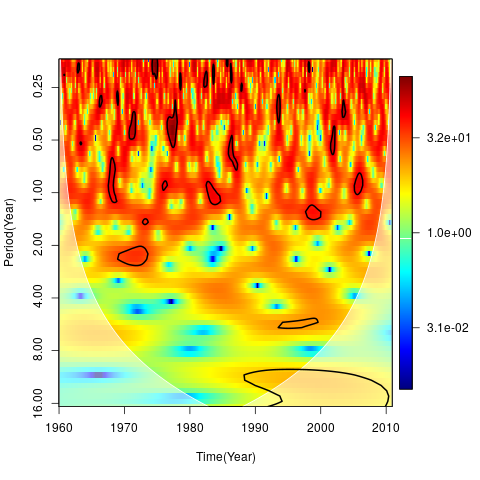
\includegraphics[width=0.7\linewidth]{wavelet}
	\caption{}
	\label{fig:wavelet}
\end{figure}

\newpage
\subsection{Detrended Wavelet}
\begin{figure}[h]
	\centering
	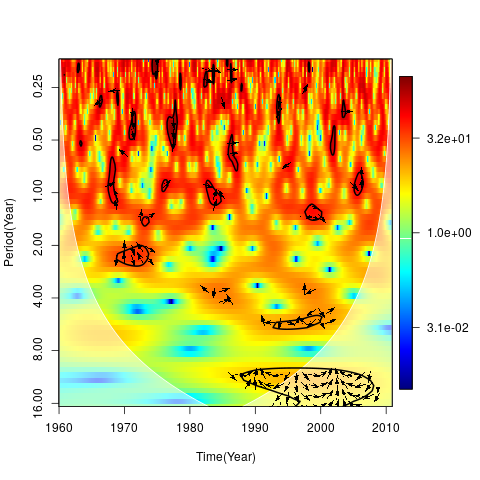
\includegraphics[width=0.7\linewidth]{waveletD}
	\caption{}
	\label{fig:waveletd}
\end{figure}
\newpage
\subsection{Coherence Wavelet}
\begin{figure}[h]
	\centering
	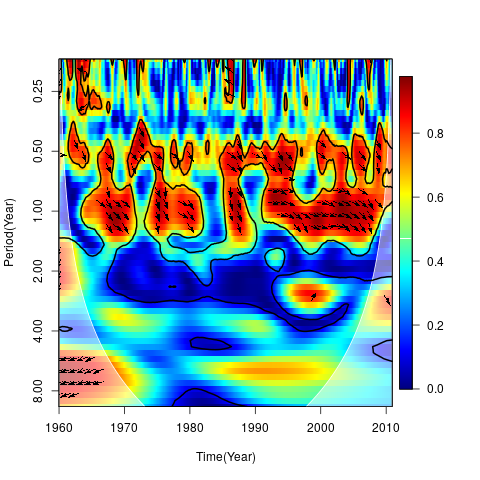
\includegraphics[width=0.7\linewidth]{wavelet_coherence}
	\caption{}
	\label{fig:waveletcoherence}
\end{figure}
\newpage
\subsection{Detrended Coherence Wavelet}
\begin{figure}[h]
	\centering
	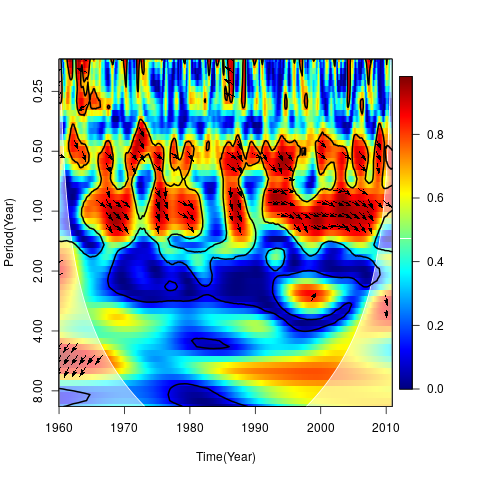
\includegraphics[width=0.7\linewidth]{wavelet_coherenceD}
	\caption{}
	\label{fig:waveletcoherenced}
\end{figure}


\end{document}